\chapter{Introduction}
\label{sec:Introduction}

Under the course unit of Integrative Project in Industrial Electronics and Computers, the students must
apply for professors' projects in order to integrate under their respective laboratories and start to understand the pace
demanded in the Master's final paper.\\

This project, given by Professor Luis Gonçalves under the CMEMS laboratory,
has the main purpose of creating a drifter for data acquisition. As a multi-themed project, this report will
explore multiple areas, as the \acrlong{pcb} design for hardware and firmware manufacture, software design under the idea to optimize
the execution, allowing for better performance. The main goal is to have the final product afloat at the end of the semester.\\



\begin{figure}[H]
    \centering
    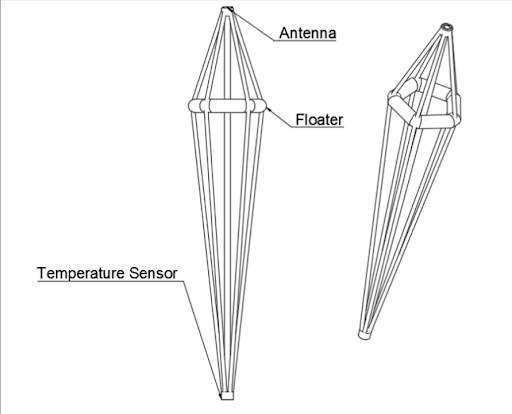
\includegraphics[width=0.7\textwidth]{images/diagrams/shell/unnamed.png}
    \caption{Draft Floater}
    \label{fig:DraftFloater}        
\end{figure}

\subsection{Problem Statement}
\label{sec:ProblemStatement}

5S, an acronym for **Sensoring System for Surface Sea Streams**, is a low-cost, low-power solution to acquire
said data with the focus to last autonomously for the longest time possible. The drifter has to attain its GPS
coordinates in order to track its current and average velocity, alongside with the water temperature and accelerometer 
information to gather data about wave intensity. All this data will be stored locally and transmitted by a protocol,
yet to be defined, using JSON format to be received by a preexisting database.  

\subsubsection{Oceanography}
\label{sec:Oceanography}

The current under study is the **Iberian Poleward Current (IPC)**, well documented by the Advanced Very High Resolution Radiometer (AVHRR)
over the last two decades. It is a narrow (25–40 km) flow of water that follows the continental slope due to topography and/or water density,
commonly referred to as a “slope-trapped tongue”. Being strongest in the winter and weaker during summer, the current is significantly warmer
and carries more salinity due to Mediterranean influence over the Eastern North Atlantic Central Water (ENACW).

\subsubsection{Transport}

It isn't uncommon to see transport accidents being reported, and even worse, for it to be a gigantic problem.
Some of these accidents are caused by poor mapping of sea conditions — tankers spilling oil, fishing vessels capsizing —
leading to financial problems and even loss of life. Even when there are no accidents, poor knowledge of tides results in higher energy consumption when routes are set against the currents.

A solution would be to create optimized shipping routes, minimizing accidents and improving energy efficiency while 
traversing the waves. Oil tankers could follow currents with lower fuel consumption. Fishing routes could become more
efficient, as their target species may swim with the tides based on temperature and speed. This would ease the workload,
making the activity less reactive and more predictable.

\begin{figure}[H]
    \centering
    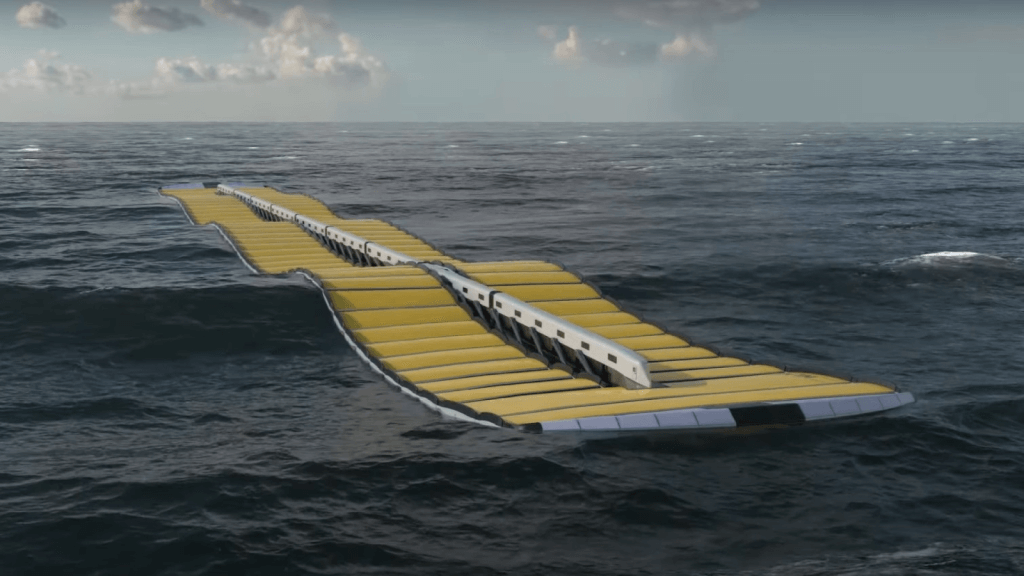
\includegraphics[width=0.7\textwidth]{images/chapter/introduction/renewable_energy.png}
    \caption{The Design of a Wave Energy Converter to Electricity}
    \label{fig:WaveEnergyConverter}        
\end{figure}

\subsubsection{Ecology}

The IPC has an important role in the ecosystem, transporting plankton, larvae, and nutrients along the coast — essential components for marine fauna and flora.

Another perspective on the importance of the IPC is in **wave energy converter placement**, a growing field of renewable energy.  
Good positioning improves efficiency and reduces costs of construction and maintenance.

\begin{figure}[H]
    \centering
    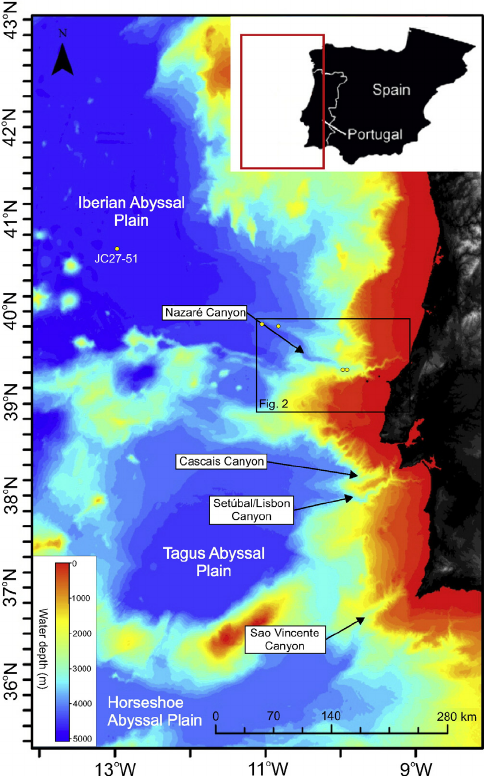
\includegraphics[angle=90,origin=c,width=0.7\textwidth]{images/maps/pt_depth.png}
    \vspace{-2.2cm}
    \caption{Depth Map of Portugal's Coast}
    \label{fig:PortugalDepthMap}        
\end{figure}

\subsubsection{Safety}

As time passes, one of the important jobs of oceanography is the study of sediments of rocky
structures at shore and their deposition. This data is useful to determine shore mineral composition,
predict erosion areas, and evaluate coastal vulnerability and resilience.

The coast attracts human activity — sports, leisure, housing, and industry — so good information around it prevents harm and fosters safety.   

\subsection{Problem Statement Analysis}
As a first step into solving this project, an initial construction of the
demends is requested. Here will be presented, following the waterfall aprouch
and UML standarts, the solutions to the individual problems presented by the project.

As stated, the floater has a series of data to acuare, format, and send in order to 
be considered concluded. The system will be divided in smaller and simpler packeges to solve
each point then it will be assembled as a final product.

\subsubsection{Equipment Objectives}
The system, in order to acomplish said targets, must set the following topics

\begin{itemize}
    \item Data acquisition
    \begin{itemize}
        \item Power Source Level \\ In order to alert a low batteries.
        \item Wave intensity \\ Measuring the force exercised by the water in the drifter
        \item Position \\ Track the movement of the water.
        \item Temperature \\ Measures the temperature directly.
    \end{itemize}
    \item Wireless data transference \\ As the floaters has no physical connections with the shore. 
    \item Local data storage \\ In case of lack of external communication.
    \item Autonomy \\ The longer it survives, the more data it will gather.
    \item Resistant and buoyant shell \\ The physical parts that support the system.
\end{itemize}




